% !TEX encoding = UTF-8 Unicode
\documentclass[a4paper]{article}
%Ovoje asdlgjsdlgkh.

\usepackage{color}
\usepackage{url}
\usepackage[T2A]{fontenc} % enable Cyrillic fonts
\usepackage[utf8]{inputenc} % make weird characters work
\usepackage{graphicx}

%\usepackage[english,serbian]{babel}
\usepackage[english,serbianc]{babel} %ukljuciti babel sa ovim opcijama, umesto gornjim, ukoliko se koristi cirilica

\usepackage[unicode]{hyperref}
\hypersetup{colorlinks,citecolor=green,filecolor=green,linkcolor=blue,urlcolor=blue}

%\newtheorem{primer}{Пример}[section] %ćirilični primer
\newtheorem{primer}{Primer}[section]

\begin{document}

\bibliographystyle{plain}
\bibstyle{plain}
\bibliography{TemaPrezime1Prezime2PrezimeN}


\title{Самсон Абрамски\\ \small{Семинарски рад у оквиру курса\\Техничко и научно писање\\ Математички факултет \\ Универзитет у Београду}}

\date{28. октобар 2019.}

\author{Александра Лабовић \\ mi19150@alas.matf.bg.ac.rs \and
	Игор Пајић \\ mi19152@alas.matf.bg.ac.rs \and
	Александар Урошевић \\ mi19201@alas.matf.bg.ac.rs \and
	Вељко Продан \\ mi19163@alas.matf.bg.ac.rs }

\begin{center}
\maketitle
\end{center}

\abstract{\textbf{Самсон Абрамски} (рођен 12. марта 1953.)\cite{pub} је информатичар са професуром Кристифора Странчеја на институту информатике Универзитета у Оксфорду. Допринео је областима теорије домена, ламбда рачунa, анализи строгости функција, теорија паралелности, категорије интеракција, геометрије интеракције, семантика игара и квантних рачунара.\cite{sa} \cite{sam} \cite{lin} \cite{log} \cite{rad} \cite{ram} }

\tableofcontents

\newpage

\section{Образовање}
\label{sec:uvod}
Абрамски је образован у Хасмонејској гимназији за дечаке у Хендону, на Краљевском факултету у Кембриџу (дипломирао је као информатичар 1975. године, 1979. завршава магистар филозофије) и у Лондонском универзитету краљице Марије (докторат информатике 1988. са ментором Ричарда Борната).\cite{obr}

\section{Каријера и истраживања}
Године 2016. Абрамски је постао сарадник Волфсон колеџа у Оксфорду и Кристифор Странчеј професор рачунарства на Одсеку рачунарске науке на Универзитету у Оксфорду. Он је такође и члан Краљевског друштва од 2004. године. Његов истраживачки рад укључује развој семантике игара, теорију домена у логичком облику и категоричку квантну механику.

Пре тога радио је на следећим положајима:

\begin{itemize}
\item     програмер, корпорација ГЕЦ рачунари, 1976-1978
\item     предавач, Одсек за рачунарске науке и статистику, Лондонски универзитет краљице Марије, 1980-1983
\item     предавач, 1983-1988, читач, 1988-1990, професор, 1990-1995, Одсек за рачунарство, Империјални колеџ у Лондону
\item     професор теорије рачунарских наука, Универзитет у Единбургу, 1996-2000
\end{itemize}
Абрамски је имао кључну улогу у развоју семантике игара и њене примене код семантике програмских језика. Остали доприноси вредни помена укључују његов рад на теорији домена у логичком облику, ламбда рачуну, анализи строгости, теорији конкурентноости, категоријама интеракције и геометрији интеракције. Недавно је радио на високим методама квантног рачунања и информација. 
\subsection{Одабране публикације}	
Самсон Абрамски је заједно са Давом Габеијем и Т.С.Е. Мејбаумом уредник шест томова Приручника логике у рачунарској науци. 
\begin{itemize}
\item     1992. Том 1: Позадина: Математичке структуре.
\item     1992. Том 2: Позадина: Рачунарске структуре.
\item     1995. Том 3: Семантичке структуре.
\item     1995. Том 4: Семантичко моделовање.
\item     2001. Том 5: Логичке и алгебарске методе.
\item 	  Том 6: Логичке методе у рачунарској науци.
\end{itemize}

Самсон Абрамски је објавио преко двеста публикација и његов h-индекс од октобра 2019. године је 57.\cite{publ}

\begin{itemize}
\item    1986. Анализа строгости код функција вишег реда. (са Г.Л. Бурном, Ц. Ханкином). Наука о рачунарском програмирању.
\item    1990. Ламбда рачун. Теме за истраживање у функционалном програмирању.
\item    1993. Рачунарска тумачења линеарне логике. У теоријској информатици 111
\item    1994. Теорија домена. (са А. Јунгом). У приручнику за логику у информатици 3.
\item    1996. Категорије интеракција и основе куцаног паралелног програмирања. (са С. Гајом и Р. Нагарајаном). НАТО АСИ СЕРИЈА Ф, НАУКА О КОМПЈУТЕРИМА И СИСТЕМИМА 152
\item    1997. Навођење категорија интеракција. (са Д. Павловићем). Теорија категорија и информатика
\item    2002. Геометрија интеракције и линеарне комбинаторне алгебре. (са Е. Хагхвердијем и П. Скотом). Математичке структуре у информатици

\item    2003. Секвенцијалност у односу на конкурентност у играма и логици. Математичке структуре у информатици 

\end{itemize}

Неки од новијих радова Самсона Абрамског укључују: 

\begin{itemize}

\item    2013. Задовољење робустног ограничења и локалне скривене променљиве вредности у квантној механици. (са Г. Готлобом и П. Колеитисом). IJCAI 2013
\item    2012. Логичке неједнакости звона. (са Луцијеном Хардијем). У Физички преглед-{ Physical Review}- A. том 85. бр. АРТН 062114
\item    2010. Увод у категорије и категоричку логику. (са Н. Твевелексом). У Нове структуре за физику. -{New Structures for Physics}- Спрингер.

\end{itemize}
\section{Награде и почасти}
Абрамски је члан Краљевског друштва (2004.), члан Краљевског друштва Единбурга (2000.),\cite{saf} и члан Европске академије (1993.). Такође је члан Уредништва Северно холандских студија логике и основа математике, и расправа о теоријској информатици Кембриџа. 
\begin{itemize}
\item    Био је председавајући Симпозијума о логици у информатици (LiCS) (2000- 2003.), и члан је СЛИ-вог оранизационог одбора.

\item    Био је изабран за члана Асоцијације рачунарских машина (2014.) За допринос у доменима логичке форме, семантике игре, категоричке квантне механике и контекстуалне семантике
\item    Награђен је Лавлејс медаљом британског рачунарског друштва 2013.\cite{sat}
\item    Награђен је чланством сениорског истраживања Истраживачког савета за инжењеринг и физичке науке 2007.
\item    Његов рад „Домен теорије у логичкој форми” освојио је СЛИ-ву награду Тест времена за 1987. годину. Награда је представљена 2007. године
\item    Награђен је чланством сениорског истраживања Истраживачког савета за инжењеринг и физичке науке за темељне структуре и методе за квантну информатику 2007. године
\end{itemize}
Номинација Самсона Абрамског за Краљевско друштво гласи:\\

Самсон Абрамски се истиче за исконски допринос математичких темеља рачунања. Његово неприкосновено достигнуће је развој семантике игара као и теорија о рачунским процесима што излаже математичке структуре протока информација између њих. Ово је довело до моћних апликација у проучавању програмских језика, нудећи нове одлучне увиде у природу секвенцијалности, стања, контроле, и многих других рачунарских карактеристика. То сада води новом развоју рачунарских програмских анализа и верификација. Једна важна нит, која такође важи као допринос у логици, је генерализација Жирарове Геометрије интеракција, што је довело до новог жанра потпуних теорема, што карактерише „простор доказа” у логици. Пре тога, Абрамски је направио важне доприносе апстракној интерпретацији, теорије домена , ламбда ($\lambda$) рачуну и паралелности. Он наставља да осветљава широк распон тема својим креативним и оштрим увидима, радећи нешто ново, и донесећи ред и јединство постојећем раду.
\section{Слика и табела}
\label{slike_i_tabele}

\begin{primer} 
\begin{figure}[h!]
\begin{center}
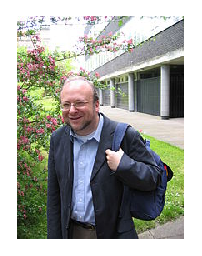
\includegraphics[scale=0.75]{abramski.eps}
\end{center}
\caption{Самсон Абрамски}
\label{fig:samson}
\end{figure}

\begin{table}[h!]
\begin{center}
\begin{tabular}{|l|l|} \hline
\textbf{Датум рођења} &12. март 1953\\ \hline
\textbf{Пребивалиште} &	Уједињено Краљевство\\ \hline
\textbf {Ментори} & Ричард Борнат\\ \hline
\end{tabular}
\label{tab:tabela1}
\end{center}
\end{table}

\end{primer}


\end{document}
